\documentclass[twocolumn, tighten, linenumbers]{aastex62}
% * <robert.stein@desy.de> 2018-05-22T07:02:06.638Z:
%
% ^.

\usepackage[latin1]{inputenc}
\usepackage{amsmath}
\usepackage{amsfonts}
\usepackage{amssymb}
\usepackage{units}
\usepackage{nicefrac}
\usepackage{graphicx}
\usepackage{hyperref}
\hypersetup{linkcolor=red,citecolor=green,filecolor=cyan,urlcolor=magenta}

\newcommand{\vdag}{(v)^\dagger}
\newcommand\aastex{AAS\TeX}
\newcommand\latex{La\TeX}

\graphicspath{{./}{figures/}}


\received{January 1, 2019}
\revised{\today}
\accepted{\today}
\submitjournal{ApJ}
\shorttitle{Search for Neutrinos from TDEs with IceCube}
\shortauthors{Stein et al.}
\watermark{DRAFT}


\begin{document}

\title{A Search for High-Energy Neutrinos from Tidal Disruption Events (TDEs) with the IceCube Neutrino Observatory}
\correspondingauthor{Robert Stein}
\email{robert.stein@desy.de}

\author{Robert Stein}
\affil{DESY Zeuthen, Platanenallee 6, 15738 Zeuthen, Germany}

\begin{abstract}
There has been much recent discussion of Tidal Disruption Events (TDEs) as potential contributors to the high-energy neutrino flux observed by IceCube, as well as possible acceleration sites for UHECRs. Here we present the first direct test of TDEs as hadronic accelerators, by searching for temporal and spatial correlation between TDEs and ten years of archival neutrino data from IceCube. We find no significant excess for either jetted TDEs or non-jetted TDEs, constraining neutrino emission for these sources. 

Under the assumption that jetted TDEs behave as standard candles, we find their isotropic-equivalent neutrino emission must be strictly less than $6 \times 10^{53} $ ergs.  Using the best-fit spectral index of the high-energy neutrino spectrum, $\gamma=-2.5$, we strongly constrain the contribution of jetted TDEs to the neutrino flux to be less that 1\%.  For a sample of reliably-identified non-jetted TDEs, we find standard-candle limit of $10^{51} $ ergs, and 26\% of the diffuse neutrino flux. Separate analyses of Swift J1644+57, Swift J2058+05, ASASSN-14li, XMMSL1 J0740-85 and AT2018cow yielded individual constraints on neutrino emission from these sources.
\end{abstract}

\keywords{neutrino astronomy, IceCube, tidal disruption events}

\section{Introduction} 
\label{sec:introduction}
The IceCube Neutrino Observatory is a cubic-kilometer array buried 1.5 km deep in glacier ice at the geographic South Pole \cite{Aartsen:2016nxy}. When neutrinos undergo charged-current  or neutral-current interactions in the ice, daughter charged leptons emit Cherenkov light that can be detected by IceCube's 5160 Digital Optical Modules (DOMs). In 2013, IceCube discovered a flux of high-energy astrophysical neutrinos \citep{Aartsen:2015knd, Aartsen:2013jdh}, and there has been an ongoing search to identify contributing sources to this flux. Unbiased all-sky searches for both time-integrated and time-dependent neutrino anisotropy have so far failed to identify any significant clustering within the neutrino flux, see e.g  \citep{Aartsen:2016oji}, ruling out a neutrino flux dominated by a few nearby sources. The consistency of this flux with an isotropic spatial distribution suggests that it has a predominantly extragalactic origin.

The lack of independently-identified neutrino sources has motivated targeted searches using multi-wavelength and multi-messenger data, seeking to identify an excess of neutrinos correlated with a known object or population. Previous searches targeting populations such as Gamma-Ray Bursts (GRBs), Fermi Blazars and Core-Collapse Supernovae (CCSNe) have also not revealed a correlation with any of the astrophysical transient or variable classes that have so far been tested. Though recent evidence has identified the flaring blazar TXS 0506+56 as a likely neutrino source \citep{IceCube:2018cha}, general limits on cumulative neutrino emission from resolved Fermi blazars as a population leave the vast majority of the diffuse flux unaccounted for. It is clear that further source classes will be required to explain the IceCube observations.

The production of high-energy neutrinos occurs through interactions of accelerated protons with either photons ($p\gamma$ interactions) or matter (pp interactions). To reach the neutrino energies in excess extending beyond 1PeV that are observed by IceCube, extreme cosmic accelerators are required. One such class of comsic accelerators that not yet been tested is the tidal disruption of stars by Supermassive Black Holes (SMBHs), so-called Tidal Disruption Events (TDEs). We here present the first test of correlation between TDEs and neutrinos, providing direct limits on the neutrino emission from both jetted and non-jetted TDEs. Our results significantly constrain models identifying jetted TDEs as a dominant source of cosmic rays.

This paper is organized as follows: Section \ref{sec:TDEs} introduces TDEs, followed by a discussion on the analysis methods in Section \ref{sec:AnalysisMethod} and the presentation of results in section \ref{sec:Results}. Section \ref{sec:DiffuseNeutrinoFlux} presents the constraints on the contribution of both jetted and non-jetted TDEs to the diffuse neutrino flux. Section \ref{sec:AT2018cow} introduces an analysis of extraordinary transient AT2018cow. Section \ref{sec:Conclusion} summarizes the paper. Upper limits on the total energy released in neutrinos from individual TDEs can be found in the Appendix \ref{sec:tde_cat}.

\section{Tidal Disruption Events}
\label{sec:TDEs}
%
%TDEs occur when a star approaches an SMBH on a plunging orbit. As the star nears the SMBH, the tidal forces acting to distort the star will increase. At a critical distance, known as the tidal radius, the tidal forces will exceed the self-gravity binding the star together, and the star will then disintegrate. After the tidal disruption, roughly one half of the stellar debris is accreted onto the black hole, while the other half becomes unbound. In an idealised case, the fallback of the stellar debris onto the SMBH along parabolic orbits will produce a characteristic $t^{-\frac{5}{3}}$ power law lightcurve. 
%
%Shortly after the idea was first proposed \cite{rees1988}, data from X-Ray surveys such as ROSITA in the 1990s began to identify lightcurves consistent with these predictions. It was not until X that a TDE was discovered while still brightening, and was first disvoered by Optical/UV. Since then, high-cadence optical surveys such as PTF, ASASSN and PanStarrs began discovering so-called "Optical TDEs" in increasing number. Following the discovery of ASASSN-14li, which was observed in optical, UV and X-Ray and Radio.

%A peculiar transient initially detected by Swift-BAT as GRB110328A was quickly revealed to be the first TDE observed with a relativistic jet. Two further TDEs were found by Swift, with all three having jets pointing towards us. These jetted TDEs are ideal environments for particle acceleration, and are consequently promising sources of both cosmic rays and neutrinos. There has been increasing interest in TDEs as a possibly-dominant source of both Ultra-High Energy Cosmic Rays (UHECRs) and high-energy neutrinos (\cite{biehl18}, \cite{daifang16} \cite{murase16} \cite{winter17}). Constraints from radio observations suggest that most TDEs do not form such relativistic jets. Nonetheless, there has theoretical studies predicting neutrino emission from TDEs without observed jets, through models invoking relativistic outflows or choked-jets. 

A TDE occurs when a star approaches an SMBH on a parabolic orbit \cite{Komossa:2015qya}. As gravitational acceleration follows a $\frac{1}{r^{2}}$ dependence, the near side of the star will be accelerated more strongly than the far side. The star thus experiences a net tidal force. As the star moves closer to the SMBH, the tidal force increases, until it exceeds the self-gravity that holds the star together. At this point the star disintegrates, and is said to be tidally-disrupted. Roughly half of the stellar debris is accreted on to the SMBH. In some cases, a relativistic jet can be formed during the accretion process, analagously to a blazar jet. There has been recent theoretical interest in TDEs as potential Ultra-High Energy Cosmic Ray (UHECR) sources, as well as candidate neutrino sources, see e.g \cite{Biehl:2017hnb}.

TDEs are a fundamentally rare phenomenon, with rates several orders of magnitude below CCSN rates \cite{vanVelzen:2017qum}. However, historically poor detection efficiencies have further exacerbated this, leaving only a handful of reliably-identified TDEs. To date, there have been only 3 on-axis jetted TDEs, and a few dozen candidate non-jetted TDEs \cite{Komossa:2015qya, Auchettl:2016qfa}. Among these, the majority do not have an unambiguous TDE classification. 

%TDEs themselves are, by their nature, nuclear transients. They can often be confused with flares of Active Galactic Nuclei (AGN), as well as nuclear CCSNe. Due to the greater abundance of these background populations, it can be hard to remove all contamination. Ultimately, muliple eras of spectroscopy and photometry are required for a compelling classification.
% At the time of catalogue compilation in October 2017 \cite{Auchettl:2016qfa}, out of approximately 60 candidate TDEs in the literature overlapping the IceCube data-taking period, only 13 were judged to be unambigouously classified. 


%\section{The Data}
%\label{sec:data}
%Neutrino-nucleon interactions in the ice are detected indirectly, via Cherenkov light emission from secondary particles, by 5160 photomultiplier tubes. While charged-current interactions of muon-neutrinos produce track-like signatures with good sub-degree angular resolution, both charged-current interactions of electron and tau neutrinos, and neutral current interactions, result in poor angular resolution. This analysis utilizes a selection of ten years of IceCube muon-track data that was optimised for point-source searches~\citep{Aartsen:2016oji}, with roughly 900,000 events from years 2008 to 2018.

Four distinct TDE catalogues were compiled as part of this analysis, using data from the OpenTDECatalog CITE, as well as data from the literature and public data from CRTS/ASASSN. From the starting point of all TDEs, two subsamples were created:

\begin{itemize}
	\item \textbf{Jetted TDEs} are X-Ray-bright TDEs which launched relativistic jets pointing towards the Earth. There are three jetted TDEs, and neutrino emission is most promising from this category
	
	\item \textbf{Obscured TDEs} are TDE candidates which occur in very dusty galaxies, and are only observed via reprocessed infra-red emission. It is unclear whether these objects are actually TDEs, with Changing-Look Active Galactic Nucleii (CLAGN) being one alternative explanation. Depending on the galaxy geometry, there would be a delay of unknown length between maximal TDE luminosity and the detected peak IR luminosity. The search window for neutrino emission from obscured TDEs is consequently much less constrained.
\end{itemize}
Of the remaining TDEs, attention was paid to the possibility of source confusion. To avoid contamination of the catalogue by missclassified AGN or SN, the remaining TDEs were further split into a golden sample of reliably-classified TDEs, and those with more ambiguous classification.
\begin{itemize}
	\item \textbf{Golden TDEs} are strong candidates where the TDE interpretation is supported by multiple spectra
	\item \textbf{Silver TDEs} are all other candidates, where a TDE interpretation is either likely or not disfavoured.
\end{itemize}

For each jetted/gold/silver TDE, an individual search window was defined for neutrino emission, according to the following criteria:

\begin{itemize}
	\item For TDEs in which the light curve was observed when rising, the first measurement is taken as the window start.
	
	\item For TDEs without an observation during lightcurve rise, the last upper limit is taken as the window start.
	
	\item The maximum date was taken as the date on which the brightest TDE luminosity measurement was performed.
	
	\item The window extends from the defined window start to 100 days after the maximum date
	
\end{itemize}

Applying these criteria gives a tailored search window for each TDE. To account for potential delay following neutrino emission, Obscured TDEs instead had a search window extending from 300 days before peak to 100 days after peak. The four catalogues, including search windows, are provided in the Appendix. It is the first such catalogue to contain time windows, and could be used for stacking analyses of e.g gamma-ray emission.

In addition, four TDEs were selected for individual analysis. Two of the three jetted TDEs, Swift J1644+57 and Swift J2058+05, were chosen due to their luminosity, as well as their position in the northern hemisphere where IceCube has the highest effective area. In addition, ASSASN-14li and  XMMSL1 J0740-85 were chosen as non-jetted TDEs which were both nearby and bright. These four TDEs were the only catalogue sources that were also detected in radio observations, typically a tracer for relativistic particle acceleration.

% 
\section{Analysis Method}
\label{sec:AnalysisMethod}
For each catalogue, a stacking analysis was performed using the same method as \cite{stasik}.
This analysis utilizes a selection of ten years of IceCube muon-track data that was optimised for point-source searches~\citep{Aartsen:2016oji}, with roughly 900,000 events from May 2008 to October 2017. 

Typical stacking analyses traditionally assume that the source class is composed of standard candles producing a uniform flux, which is then scaled with the luminosity distance and convoluted with detector acceptance to calculate the number of neutrinos that each source contributes. While this method is optimal in the case that the sources are indeed standard candles, it is generally dominated by the closest catalogue sources. Under deviations from this case, for example if a selection bias leads to more distant sources being intrinsically brighter, the standard candle assumption is not appropriate. In this work, the number of signal neutrinos was instead fitted for each source individually, so that overall the Likelihood function is a sum over many sources with one spectral index.

The signal PDF, $\mathcal{S}$, of each neutrino is evaluated as a product of energy, spatial and time PDFs. The neutrinos are assumed to follow a power law $E^{-\gamma}$, where the spectral index $\gamma$ is a fit parameter. The distribution of neutrinos from a source is assumed to be a 2D gaussian with an energy-dependent angular error, while the temporal 'neutrino light curve' is taken as a uniform box function over the search window. These terms are convoluted with the energy-dependent detector acceptance, which also evolves between data-taking seasons. 

As the IceCube datasets are dominated by atmospheric muon and muon-neutrino background, data-based PDFs used to evaluate the background PDF, $\mathcal{B}$,  of neutrinos. The energy and spatial PDFs are comprised of splines fitted to observed distributions, while the background rate is assumed to be uniform within data-taking seasons. Signal PDFs are constructed using simulated              Monte Carlo events.

From the definitions of $\mathcal{S}$ and $\mathcal{B}$, we can define a test statistic (TS):
\begin{equation*}
\lambda = 2\times \log \left( \frac{\mathcal{L}(\hat{n}_\text{s}, \hat{\gamma})}{\mathcal{L}(n_{s}=0)} \right)
\end{equation*}
where $\mathcal{L}(\hat{n}_\text{s}, \hat{\gamma})$ corresponds to the maximum of the likelihood function and $\mathcal{L}(0)$ to the null hypothesis, i.e.~ the case of no spatial and temporal correlation of neutrinos and TDEs~\citep{Braun:2008bg, Braun:2009aa}. 

For a given IceCube dataset, randomly scrambling each neutrino's right ascension and arrival time removes any signal clustering. Performing a likelihood ratio test on many scrambled datasets gives an estimate of the background TS distribution, which is typically a sum of a $\delta $ -function and a $\chi^{2}$ distribution. The p-value of any TS value can be evaluated as $p = \int_{\lambda_\text{exp}}^\infty \mathrm{d}\lambda$.

For each of the four individual TDEs, searches were conducted for neutrino clustering in both time and space (see e.g \cite{IceCube:2018cha}). With the spatial and energy PDFs, all 'significant' neutrinos with $\frac{\mathcal{S}}{\mathcal{B}} \geq 1$ were identified. For each unique neutrino pair, a likelihood ratio test was performed as above assuming a uniform neutrino lightcurve between the pair arrival times. To account for the higher number of possible pairs with short periods relative to longer ones, a marginalisation term is introduced and the test statistic is defined as:

\begin{equation*}
\lambda = 2\times \log \left( \frac{\mathcal{L}(\hat{n}_\text{s}, \hat{\gamma})}{\mathcal{L}(0)} \frac{T_{pair}}{T_{window}}\right)
\end{equation*}

where $T_{pair}$ is the detector livetime between the two neutrino arrival times, and $T_{window}$ is the search window length in detector livetime.

Of all tested pairs, that with the largest TS value is selected as the 'neutrino flare'. The significance of a TS value is again calculated from background-scrambled TS distributions. As can be seen in Figure \ref{fig:DiscTime}, for a short neutrino flare lying within a larger search window, the threshold neutrino fluence for discovery is significantly lower than with a traditional time-integration method.

\begin{figure}[!ht]
	\centering 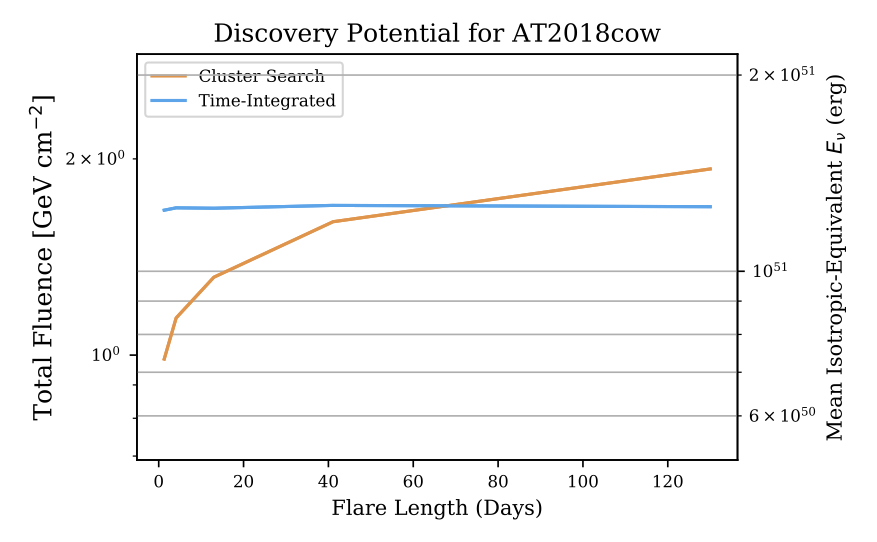
\includegraphics[width=0.48\textwidth]{figures/flare_vs_box_disc}
	\caption{The $5\sigma$ Discovery Potential for AT2018cow, in both total fluence and isotropic-equivalent energy, as a function of flare length. The analysis tests flares within a pre-defined 130 day window. For flares much shorter than the search window, significantly less fluence is required to make a discovery with the cluster-search than for a time-integrated analysis.}
	\label{fig:DiscTime}
\end{figure}

All stacking tests are described in Table \ref{tab:stacking_tests}, and all single-object tests are described in Table \ref{tab:single_tests}.

\begin{table*}[]
	\centering
	\begin{tabular}{||c c c c | c||} 
		\hline
		Catalogue & Source Class & Size & Description  & Pre-trial p-value\\ [0.5ex] 
		\hline\hline
		Jetted & Jetted TDEs &  3 & \textit{Probable TDEs with on-axis jets} & 0.44\\ 
		\hline
		Golden & Non-Jetted TDEs & 13 & \textit{Probable TDEs with convincing classification}&1.0\\
		\hline
		Silver & Non-Jetted TDEs & 24 & \textit{Candidate TDEs with ambiguous classification}&1.0\\
		\hline
		Obscured & Non-Jetted TDEs & 13 & \textit{Candidate TDEs in dusty galaxies}&0.07\\[1ex] 
		\hline
	\end{tabular}
	\caption{Summary of the four TDE catalogues. For each, an independent stacking analysis was performed. The catalogues covered sources from May 2008 to October 2017, matching the IceCube data-taking period.}
	\label{tab:stacking_tests}
\end{table*}{}

\begin{table*}[]
	\centering
	\begin{tabular}{||c c c| c |} 
		\hline
		Object & Stacking Catalogue &  Isotropic-Equivalent Energy (ergs) & Pre-trial p-value\\ [0.5ex] 
		\hline\hline
		Swift J1655+57 & Jetted TDEs & $<2 \times 10^{54}$ & 1.0\\ 
		\hline
		Swift J2058+05 & Jetted TDEs & $<2 \times 10^{51}$& 0.38\\
		\hline
		ASASSN-14li & Non-jetted TDEs (Gold) & $<2 \times 10^{51}$& 1.0\\
		\hline
		XMMSL1 J0740-85 & Non-jetted TDEs (Gold)& $<2 \times 10^{51}$ & 0.22\\
		\hline
		\hline
		AT2018cow & - & $<2 \times 10^{51}$& ??\\
		[1ex] 
		\hline
	\end{tabular}
	\caption{Summary of the five individual TDEs for which the temporal-cluster-search method was applied. All but AT2018cow were included in the stacking analysis.}
	\label{tab:single_tests}
\end{table*}{}

\section{Results}
\label{sec:Results}
Final p-values for each TDE catalogue, as well the four individual TDEs, are sumarised in Table A. The most significant result was obtained for Z. All values are consistent with those expected from background fluctuations, so no discovery is claimed. Instead we place upper limits on neutrino fluence from each catalogue and source. This is done in Figures \ref{fig:gold_flux} and \ref{fig:jetted_flux}  as a function of spectral index.

\begin{figure}[!ht]
	\centering 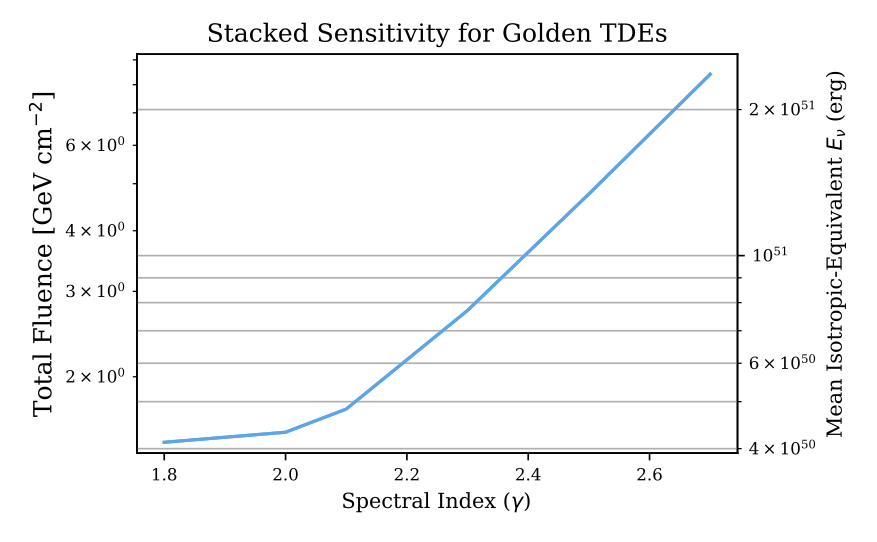
\includegraphics[width=0.45\textwidth]{figures/gold_flux}
	\caption{Limits on the neutrino energy emitted by non-jetted TDEs as a function of spectral index, under the assumption of an unbroken power law between 100 GeV and 10 PeV. This limit is derived using the golden TDE sample, under the assumption that non-jetted TDEs are neutrino standard candles and emit isotropically.}
	\label{fig:gold_flux}
\end{figure}

\begin{figure}[!ht]
	\centering 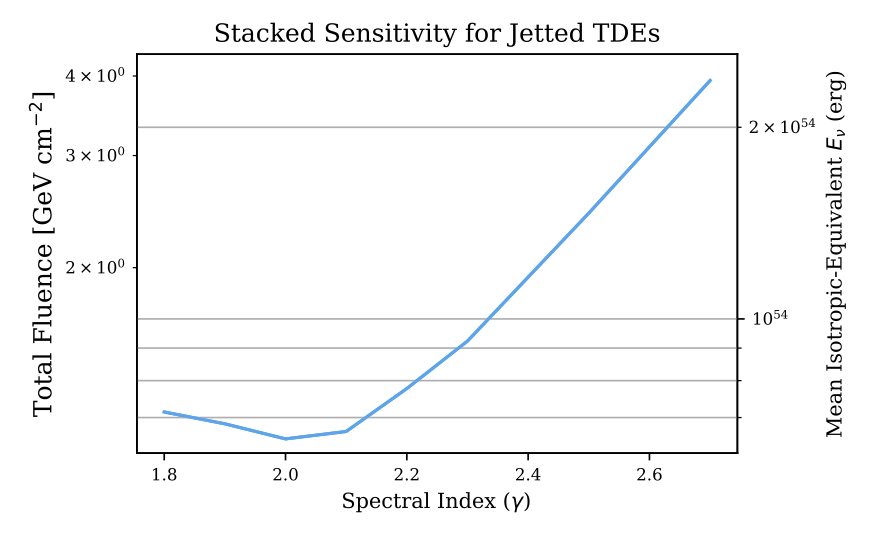
\includegraphics[width=0.45\textwidth]{figures/jetted_flux}
	\caption{Limits on the isotropic-equivalent neutrino energy emitted by jetted TDEs as a function of spectral index, under the assumption of an unbroken power law between 100 GeV and 10 PeV. This limit is derived under the assumption that jetted TDEs are neutrino standard candles.}
	\label{fig:jetted_flux}
\end{figure}

As the likelihood tests made no assumptions for the relative brightness of each source, our results can be used to constrain a variety of emission distributions. Under the simplest assumption, we assume that each TDE is an equally neutrino-bright standard candle, and thus their contribution to the neutrino flux on Earth is simply proportional to $\frac{1}{D_{L}(Z)^{2}}$. 

As the Golden catalogue candidates were selected based on their strong likelihood of being genuine TDEs, the corresponding limits derived for the entire non-jetted TDE population can be considered robust. However, given the likely sample contamination, we do not attempt to similarly extrapolate results from silver or obscured samples to non-jetted TDEs as a population.

\section{Diffuse Neutrino Flux}
\label{sec:DiffuseNeutrinoFlux}

From the per-source limits derived in Figures \ref{fig:gold_flux} and \ref{fig:jetted_flux}, we can derive limits on the cumulative neutrino emission from non-jetted and jetted TDEs as populations. To do this, we calculate the rate of TDEs as a function of redshift, assuming a local rate and a source evolution derived in y. We then numerically integrate the flux contributed by shells of increasing redshift up to a horizon of z=8, to calculate the cumulative flux expected for each population. This method thus accounts for TDEs that were not detected by other surveys, and were therefore not incorporated into our catalogue.

To perform this calculation, we use the most recent IceCube global fit of the astrophysical neutrino flux, with a best-fit spectrum of $E^{-2.50}$ and normalisation of X at 100 TeV. For non-jetted TDEs, we assume a central local rate of $8 \times 10^{-7}$ Mpc$^{-3}$ year$^{-1}$ \citep{vanVelzen:2017qum}, a source evolution derived by \cite{Sun:2015bda}, and constrain the contribution of TDEs to be less than 26\% of the total. For jetted TDEs, under the assumption that they follow the same underlying source evolution as non-jetted TDEs with a central rate of $3 \times 10^{-11}$ Mpc$^{-3}$ year$^{-1}$ \citep{Sun:2015bda}, we find that they must contribute less than 1\% of the total.  These constraints are illustrated in Figure \ref{fig:DiffuseFlux}.

\begin{figure}[!ht]
	\centering 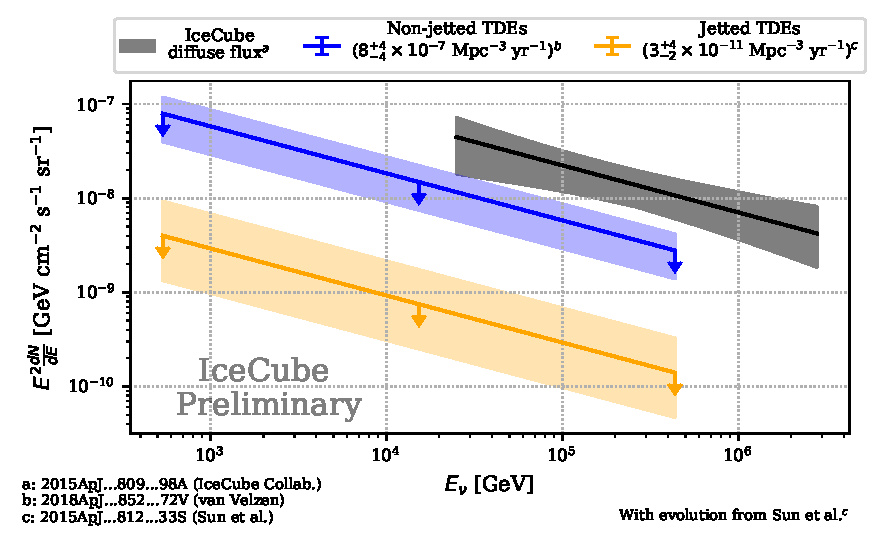
\includegraphics[width=0.45\textwidth]{figures/diffuse_flux_global_fit}
	\caption{Limits on the contribution of jetted and non-jetted TDEs to the diffuse neutrino flux, assuming standard candle behaviour. The shaded bands represent uncertainty in local rate estimates.}
	\label{fig:DiffuseFlux}
\end{figure}

As the contribution from a population is directly proportional to the local population rate, the shaded bands indicate the uncertainty in our limits arising from rate estimates. For TDEs, these rates are the dominant source of uncertainty in neutrino flux. It will require systematic evaluation of observed TDE rates to enable more precise limits on neutrino emission. Any refined rate estimate can be used to linearly rescale these limits. Propagating through the current local rate uncertainty, we constrain non-jetted TDEs to be less than 13-39\%, and jetted TDEs to be less than 0.n-1.n\% of the total.

\section{AT2018cow}
\label{sec:AT2018cow}
Following the four stacking analyses and four object analyses described in Section \ref{sec:AnalysisMethod}, an additional analysis was performed on AT2018cow. This object
 was a fast, bright, blue transient first discovered in 2018 cite. The observations suggested AT2018cow was a nearby example of a recently-identified population of Fast Blue Optical Transients (FBOTs) \cite{Margutti:2018rri}. 

Shortly after the time of discovery, AT2018cow was thought to be a Broad-Lined type IC (IC-BL) supernova, and thus a member of the rare CCSN subclass associated with long GRBs and choked-jets CITE. As many models predict that such SNe may be neutrino sources, an IceCube Fast Reponse Analysis was run on AT2018cow shortly after discovery CITE. Within the context of a candidate choked-jet supernova, the IceCube search focussed on the period spanning the 3-day period from the last non-detection to the first detection, aiming to isolate the supernova explosion time at which the neutrino emission would be expected. Ultimately, an excess of neutrinos was found in this time period, with a significance of 1.8 $\sigma$ \citep{2018ATel11785....1B}. The excess itself consisted of two signal-like neutrinos, which were considered significant owing to the small expected background for such a short search window.

Later multi-wavelength observations of AT2018cow were not consistent with a traditional IC-BL SN, and the transient has since variously interpreted as a TDE, an extreme SN or a Magnetar \citep{Perley:2018oky}. In light of these developments, AT2018cow was re-analysed by IceCube in the context of a potential TDE classification. As for the other four individual TDEs, a dedicated search for neutrino clustering on timescales up to 130 days, extending from 30 days before peak to 100 days afterwards, was undertaken.  For this purpose, an additional year of IceCube data extending to October 2018 was analysed.

In this analysis of AT2018cow, a small excess was again found. Although the best-fit cluster from this search included the two signal-like neutrinos from the original IceCube analysis, when accounting for the expected fluctuations arising from background over the much longer 130 day search window, the significance of the excess was just 0.5 $\sigma$. The results are thus entirely consistent with expectations from atmospheric background, while not contradicting the original result published at the time. As such, no discovery is claimed and upper limits are accordingly derived (illustrated in Figure \ref{fig:At2018cow}). We emphasize that AT2018cow was not included in our catalogues at the time when the stacking analysis was performed, but would naturally belong to the silver non-jetted TDE sample. This object will be included in a future analysis incorporating more years of IceCube data.

\begin{figure}[!ht]
	\centering 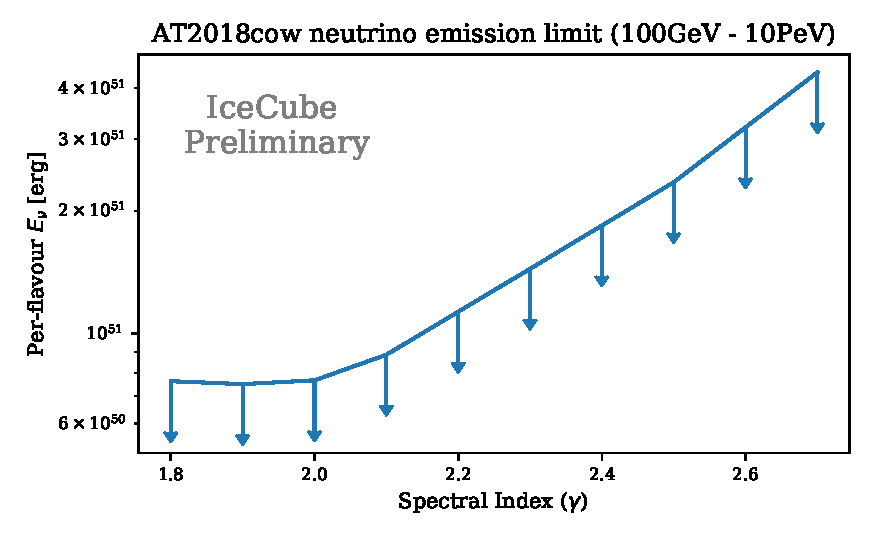
\includegraphics[width=.45\textwidth]{figures/AT2018cow_limit_plot}
	\caption{Limits on integrated neutrino emission from AT2018cow as a function of spectral index, assuming a 130 day window from MJD 58256.9 to MJD 58386.9}
	\label{fig:At2018cow}
\end{figure}


\section{Conclusion}
\label{sec:Conclusion}
We have here presented the first search for neutrinos from TDEs with IceCube. In a stacking analysis we tested correlations between dozens of TDEs and approximately 900000 muon-track events. No significant correlation was found with either jetted, or non-jetted TDEs.

Non-jetted and Jetted TDEs contribute less than 26\% and 1\% respectively to the astrophysical neutrino flux at the $90\%$ confidence level, assuming an unbroken power law with index -2.5. Separate analyses of individual objects did not reveal any significant neutrino emission from Swift J1644+57, ASASSN-14li or AT2018cow.

Improvements of the presented limits are expected in the near future with novel optical survey instruments such as the Zwicky Transient Factory (ZTF) \citep{2014htu..conf...27B} (TO BE REPLACED BY NEW REF) which is undertaking a high-cadence survey across a large fraction of the sky. ZTF is discovering a substantial number of TDEs, and these objects have well-sampled lightcurves that will provide better-constrained search windows.

\bibliography{my-bib-database}
\addcontentsline{toc}{chapter}{Bibliography}

\appendix

\section{TDE Catalogues}
\label{sec:tde_cat}

\subsection{Jetted TDEs}

\begin{table*}
	\centering
\begin{tabular}{||c c c c ccc|} 
	\hline
	Object & Right Ascension &  Declination  & Luminosity Distance & $T_{start}$ & $T_{End}$ & Reference\\ [0.5ex] 
	& (deg.) & (deg.) & (Mpc) &(MJD) & (MJD) &\\
	\hline\hline
	Swift J1655+57 & Jetted TDEs & && 1.0\\ 
	\hline
	Swift J2058+XX & Jetted TDEs & & & 0.38\\[1ex] 
	\hline
\end{tabular}
\caption{Summary of the three jetted TDEs.}
\label{tab:jetted_cat}
\end{table*}

\begin{table*}
	\centering
	\begin{tabular}{||c c c c ccc|} 
		\hline
		Object & Right Ascension &  Declination  & Luminosity Distance & $T_{start}$ & $T_{End}$ & Reference\\ [0.5ex] 
		& (deg.) & (deg.) & (Mpc) &(MJD) & (MJD) &\\
		\hline\hline
		Swift J1655+57 & Jetted TDEs & && 1.0\\ 
		\hline
		Swift J2058+XX & Jetted TDEs & & & 0.38\\[1ex] 
		\hline
	\end{tabular}
	\caption{Summary of the twelve golden non-jetted TDEs.}
	\label{tab:gold_cat}
\end{table*}

\end{document}


